\documentclass[11pt,a4paper]{report}
\usepackage[toc,page]{appendix}
\usepackage{multirow}
\usepackage[utf8]{inputenc}
\usepackage[english]{babel}
\usepackage{amsmath}
\usepackage{amsfonts}
\usepackage{amssymb}
\usepackage{graphicx}
\author{Hämäläinen, Harri \\
\texttt{harri.hamalainen@aalto.fi}
\and
Islam, Hasan \\
\texttt{hasan.islam@aalto.fi}
\and
Kurnikov, Arseny \\
\texttt{arseny.kurnikov@aalto.fi}}
\title{S-38.3159 Protocol Design: Final evaluation of implementation}
\begin{document}
\maketitle

\chapter{Evaluation}

This report will assemble all of test results for IoT pub/sub protocol implementation. This report will be decomposed into six parts; Test one to six. Task one and two will be studied in ideal scenario, Task three and four will focus on reliability issues. The report will present freshness, delay and loss metric. In tasks five and six we will study the congestion and its effect on the protocol performance. Our implementation have own Markovian Packet Loss Generator. 

\chapter{Test 1}

\hspace*{4.3mm} \textit{Scenario:} 1 client connect to all sensors

\textit{Environment:} No losses, delays or b/w restrictions

\begin{center}
\begin{table}[h]\footnotesize
  \begin{tabular}{| p{3cm}  | p{1.5cm} | p{1.5cm} | p{2cm} |p{1cm} |}
   \hline
  \textbf{Client}  & \textbf{Camera} & \textbf{Device} & \textbf{Temperature} & \textbf{GPS}\\ \hline
   Mean Delay & 0 & 0 &  0 &  0 \\ \hline
   Max Delay & 0 &0  & 0  & 0  \\ \hline
   Min Delay  & 0 &  0& 0  & 0  \\ \hline
   Variance Delay  & 0 & 0 & 0  & 0  \\ \hline
  \end{tabular}
   \caption{Scheduling and Load Distribution.}
    \label{comparison}  
  \end{table}
\end{center}

\chapter{Test 5: Congestion control}
In tasks five and six we study the congestion and its effect on the protocol
performance. In order to provide reliable transport while not contributing to
congestion collapse many protocols provide or use different mechanisms for congestion control and
flow control. In this section we study the effect of heterogeneous bandwidth in
different configurations our protocol implementation supports.

\section{Evaluation scenario}
To evaluate the performance under the assumptions given in this task four clients
were assigned a IP address from loopback address block (127.0.0.0/8). The server
belongs also to this address block. This network setup of ours is given in
figure \ref{fig:task5-setup}.  These additional addresses were created as
alises with command:\\
\\
\texttt{sudo ifconfig lo0 alias 127.0.0.2}
\\

Dummynet was used to create link characteristics between client and server
machines with e.g. following command for each link between client and server
(naturally changing the IP addresses as required): \\ 
\\
\texttt{sudo ipfw add pipe 1 ip from 127.0.0.2 to 127.0.0.10; \\sudo ipfw pipe 1 config bw 500kb }

\begin{figure}
\centering
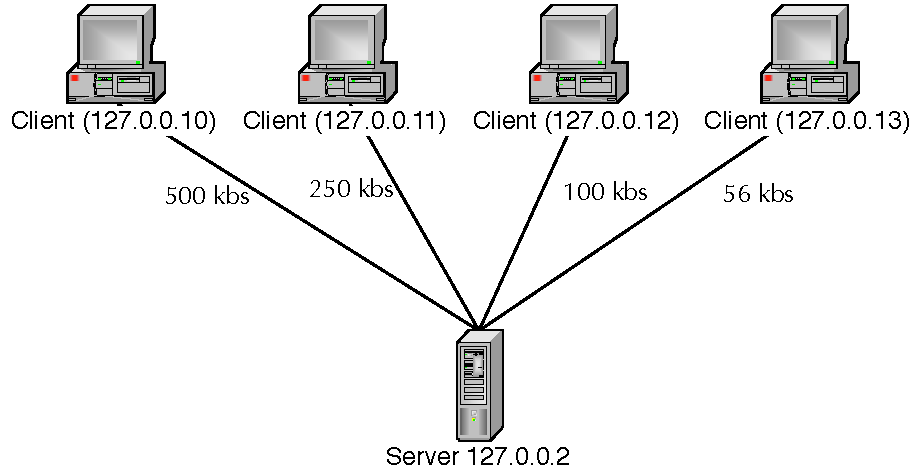
\includegraphics[scale=0.5]{task5-setup.pdf} 
\caption{Number of flows with given flow timeout values}
\label{fig:task5-setup}
\end{figure}

\section{Results}

In table \ref{table:task5-camera-a} the delay statistics and packet loss is
shown for the case where the connections are created without a reliability
guarantees and without any kind of congestion control. 

In table \ref{table:task5-camera-b} the weakly reliable transport is used for
all connections. We see a large increase of packet losses when reliability is
turned on. The reason for this counter intuitive behaviour is most likely due to
camera sensors which have high traffic volumes. In the appendix
\ref{appendix:task5} we see that for low traffic temperature sensors the
weakly reliable transport means less packet losses.

In table \ref{table:task5-camera-c} the results when no reliability guarantees are given but the simple
congestion control mechanism is used.

Finally we show the results when both weakly reliable transport is combined with
simple congestion control in table \ref{table:task5-camera-d}.



In comparison to high traffic volume sensors the results for temperature sensors
are given in appendix.

\begin{table}
\centering
\begin{tabular}{|c|c|c|c|c|c|c|c|c|}
\hline
client & E[D] & max(D) & min(D) & Var(D) & E[s] & max(s) & Var(s) & plr\\
\hline
500kbs & 0.024 & 0.079 & 0 & 0.0001 &  0.067 & 1 & 0.064 & 0\\
\hline
250kbs & 0.047 & 0.100 & 0 & 0.0003 &  0.102 & 1 & 0.093 & 0\\
\hline
100kbs & 0.728 & 1.670 & 0.0199 & 0.186 & 2.203 & 11 & 13.854 & 0.038 \\
\hline
56kbs & 1.935 & 3.950 & 0.0299 & 1.217 & 6.119 & 22 & 48.279 & 0.147 \\
\hline
\end{tabular}
\caption{Task 5: Receive statistics (delay[D], skew[s], packet loss rate [plr]) for camera sensor data (no realibility guarantees, no congestion control)}
\label{table:task5-camera-a}
\end{table}


\begin{table}
\centering
\begin{tabular}{|c|c|c|c|c|c|c|c|c|}
\hline
client & E[D] & max(D) & min(D) & Var(D) & E[s] & max(s) & Var(s) & plr\\
\hline
1 (500kbs) & 0.022 & 0.040 & 0.000 & 0.000 & 0.019 & 1.000 & 0.019 & 0\\
\hline
2 (250kbs) & 0.044 & 0.080 & 0.000 & 0.000 & 0.056 & 1.000 & 0.053 & 0\\
\hline
3 (100kbs) & 0.730 & 2.040 & 0.010 & 0.215 & 3.407 & 34.000 & 41.755 & 0.24\\
\hline
4 (56kbs) & 1.487 & 3.110 & 0.200 & 0.568 & 7.093 & 34.000 & 91.142 & 0.65\\
\hline
\end{tabular}
\caption{Task 5: Receive statistics (delay[D], skew[s], packet loss rate [plr]) for camera sensor data (weakly realible transport, no congestion control)}
\label{table:task5-camera-b}
\end{table}


\begin{table}
\centering
\begin{tabular}{|c|c|c|c|c|c|c|c|c|}
\hline
client & E[D] & max(D) & min(D) & Var(D) & E[s] & max(s) & Var(s) & plr\\
\hline
1 (500kbs) & 0.024 & 0.060 & 0.000 & 0.000 & 0.115 & 1.000 & 0.104 & 0\\
\hline
2 (250kbs) & 0.047 & 0.090 & 0.000 & 0.000 & 0.135 & 1.000 & 0.119 & 0\\
\hline
3 (100kbs) & 0.742 & 1.800 & 0.010 & 0.185 & 2.115 & 12.000 & 12.339 & 0 \\
\hline
4 (56kbs) & 1.972 & 4.090 & 0.020 & 1.085 & 6.231 & 27.000 & 51.985 & 0 \\
\hline
\end{tabular}
\caption{Task 5: Receive statistics (delay[D], skew[s], packet loss rate [plr]) for camera sensor data (no reliability guarantees, skipping messages)}
\label{table:task5-camera-c}
\end{table}


\begin{table}
\centering
\begin{tabular}{|c|c|c|c|c|c|c|c|c|}
\hline
client & E[D] & max(D) & min(D) & Var(D) & E[s] & max(s) & Var(s) & plr\\
\hline
1 (500kbs) & 0.022 & 0.040 & 0.000 & 0.000 & 0.051 & 1.000 & 0.049 & 0\\
\hline
2 (250kbs) & 0.044 & 0.080 & 0.000 & 0.000 & 0.102 & 1.000 & 0.093 & 0\\
\hline
3 (100kbs) & 0.710 & 1.640 & 0.010 & 0.201 & 1.322 & 12.000 & 9.601 & 0.11\\
\hline
4 (56kbs) & 1.356 & 2.760 & 0.020 & 0.718 & 4.000 & 27.000 & 60.690 & 0.59\\
\hline
\end{tabular}
\caption{Task 5: Receive statistics (delay[D], skew[s], packet loss rate [plr]) for camera sensor data (weakly reliable transport, skipping messages)}
\label{table:task5-camera-d}
\end{table}


\chapter{Test 6: Congestion control and Reliability}
In this section we study the effect of heterogeneous bandwidth with different
packet loss rates in different configurations our protocol implementation supports.

\section{Evaluation scenario}
To evaluate the performance under the assumptions given in this task four clients
were assigned a IP address from loopback address block (127.0.0.0/8). The server
belongs also to this address block. This network setup of ours is given in
figure \ref{fig:task5-setup}.  These additional addresses were created as
alises with command:\\
\\
\texttt{sudo ifconfig lo0 alias 127.0.0.2}
\\

Dummynet was used to create link characteristics between client and server
machines with e.g. following command for each link between client and server
(naturally changing the IP addresses as required): \\ 
\\
\texttt{sudo ipfw add pipe 1 ip from 127.0.0.2 to 127.0.0.10; \\sudo ipfw pipe 1 config bw 500kb }
\\
The packet loss was created with our transport layer implementation which is
capable to simulate artificial packet loss and delays. It's good to notice
however that this is not the most realistic situation as packet loss is only
happening on the link from server to client. This means that when a weakly
realiabile subscriptions are used all acknowledgements are not experiencing any
packet loss except in case that happens naturally. The loss rates for clients
are 0.15 and 0.05. The losses are bursty meaning that when a loss happens it's
more likely that also the next message will be lost.

In comparison to high traffic volume sensors the results for temperature sensors
are given in appendix \ref{appendix:task6}.

\section{Results}
The scenario where we have no weak-reliability guarantees or active congestion
control are shown in table \ref{table:task6-camera-a} for camera sensor data. We
observe quite high packet loss rate due to fragmentation while also the effect
of bandwidth is clearly shown.

The results when weakly reliable connections are used are shown in table
\ref{table:task6-camera-b}. We see no improvement in packet losses which is
likely due to high traffic volume of the camera sensors. Because of this the
sensor updates which are lost are going to be retransmitted while due to burstly
updates from camera most likely cause the messages to be short lived.
Retransmitting short lived messages like camera updates are bad thing with our
current implementation because this blocks the transmission of newer updates as
the server is not threaded.

The statistics when message skipping is turned on are shown in table
\ref{table:task6-camera-c}. As assumed the skipping does not provide any good
mean to prevent the congestion effects. The statistics when message skipping is turned on with weakly reliable transport are shown in table
\ref{table:task6-camera-d}.

The results for temperature sensors (shown in appendix \ref{appendix:task6})
show that the reliable connections are working properly (packet loss is
minimized) when the communication flow has low traffic intensity.


\begin{table}
\centering
\begin{tabular}{|c|c|c|c|c|c|c|c|c|}
\hline
client & E[D] & max(D) & min(D) & Var(D) & E[s] & max(s) & Var(s) & plr\\
\hline
500kbs 0.05 & 0.044 & 0.080 & 0.000 & 0.000 & 0.390 & 2.000 & 0.345 & 0.16\\
\hline
500kbs 0.15 & 0.044 & 0.070 & 0.000 & 0.000 & 2.203 & 13.000 &9.751 & 0 0.5 \\
\hline
100kbs 0.05 & 2.336 & 4.350 & 0.100 & 1.523 & 8.407 & 25.000 & 65.970 & 0.35 \\
\hline
100kbs 0.15 & 1.323 & 2.590 & 0.020 & 0.506 & 5.085 & 21.000 & 34.838 & 0.55 \\
\hline
\end{tabular}
\caption{Task 6: Receive statistics for camera sensor data (no realibility guarantees, no congestion control)}
\label{table:task6-camera-a}
\end{table}

\begin{table}
\centering
\begin{tabular}{|c|c|c|c|c|c|c|c|c|}
\hline
client & E[D] & max(D) & min(D) & Var(D) & E[s] & max(s) & Var(s) & plr\\
\hline
500kbs 0.05 & 0.044 & 0.080 & 0.000 & 0.000 & 0.153 & 2.000 & 0.166 & 0.18 \\
\hline
500kbs 0.15 & 0.060 & 0.660 & 0.000 & 0.007 & 0.339 & 6.000 & 1.021 & 0.54 \\
\hline
100kbs 0.05 & 2.050 & 3.070 & 0.520 & 0.530 & 5.085 & 26.000 & 61.286 & 0.70 \\
\hline
100kbs 0.15 & 1.100 & 2.120 & 0.030 & 0.323 & 3.237 & 26.000 & 38.943 & 0.76 \\
\hline
\end{tabular}
\caption{Task 6: Receive statistics for camera sensor data (weakly reliable transport, no congestion control)}
\label{table:task6-camera-b}
\end{table}


\begin{table}
\centering
\begin{tabular}{|c|c|c|c|c|c|c|c|c|}
\hline
client & E[D] & max(D) & min(D) & Var(D) & E[s] & max(s) & Var(s) & plr\\
\hline
500kbs 0.05 & 0.045 & 0.080 & 0.000 & 0.000 & 2.145 & 5.000 & 3.090 & 0.31\\
\hline 
500kbs 0.15 & 0.038 & 0.070 & 0.000 & 0.000 & 0.545 & 6.000 & 1.438 & 0.59\\
\hline
100kbs 0.05 & 2.625 & 3.860 & 0.030 & 1.503 & 5.145 & 35.000 & 91.201 & 0.33\\
\hline
100kbs 0.15 & 2.508 & 4.210 & 0.020 & 2.044 & 4.727 & 34.000 & 88.869 & 0.42\\
\hline
\end{tabular}
\caption{Task 6: Receive statistics for camera sensor data (no reliability guarantees,transport, skipping messages)}
\label{table:task6-camera-c}
\end{table}



\begin{table}
\centering
\begin{tabular}{|c|c|c|c|c|c|c|c|c|}
\hline
client & E[D] & max(D) & min(D) & Var(D) & E[s] & max(s) & Var(s) & plr\\
\hline
500kbs 0.05 & 0.045 & 0.380 & 0.000 & 0.001 & 0.220 & 5.000 & 0.554 & 0.19\\
\hline 
500kbs 0.15 & 0.046 & 0.300 & 0.000 & 0.002 & 0.458 & 8.000 &  2.149 & 0.44\\
\hline
100kbs 0.05 & 1.738 & 3.200 & 0.030 & 0.902 & 5.983 & 28.000 & 78.362 & 0.75\\
\hline
100kbs 0.15 & 1.650 & 2.920 & 0.150 & 0.607 & 5.492 & 28.000 & 74.875 & 0.74\\
\hline
\end{tabular}
\caption{Task 6: Receive statistics for camera sensor data (weakly reliable transport, skipping messages)}
\label{table:task6-camera-d}
\end{table}

\chapter{Results for tests 1-4}
\section*{Test 1}
\begin{verbatim}
 Sensor camera_3 
Server got 23 out of 23 
client1 lost 0 out of 23 
client1 duplicated (possibly fragments) 0 
client1 out of order 0 
 mean delay 0 
 max delay 0 
 min delay 0 
 variance delay 0 
-------------------------
Sensor device_0 
Server got 12 out of 12 
client1 lost 0 out of 12 
client1 duplicated (possibly fragments) 0 
client1 out of order 0 
 mean delay 0 
 max delay 0 
 min delay 0 
 variance delay 0 
-------------------------
Sensor gps_2 
Server got 5 out of 5 
client1 lost 0 out of 5 
client1 duplicated (possibly fragments) 0 
client1 out of order 0 
 mean delay 0 
 max delay 0 
 min delay 0 
 variance delay 0 
-------------------------
Sensor temp_1 
Server got 30 out of 30 
client1 lost 0 out of 30 
client1 duplicated (possibly fragments) 0 
client1 out of order 0 
 mean delay 0 
 max delay 0 
 min delay 0 
 variance delay 0 
-------------------------
\end{verbatim}



\section*{Test 2}

\hspace*{4.3mm} \textit{Scenario:} N client connect to all sensors

\textit{Environment:} No losses, delays or b/w restrictions

\begin{verbatim}
Sensor camera_3 
Server got 86 out of 86 
client1 lost 0 out of 86 
client1 duplicated (possibly fragments) 0 
client1 out of order 0 
 mean delay 0.0008139527 
 max delay 0.00999999 
 min delay 0 
 variance delay 7.564965e-06 
client2 lost 0 out of 86 
client2 duplicated (possibly fragments) 0 
client2 out of order 0 
 mean delay 0.0005813948 
 max delay 0.00999999 
 min delay 0 
 variance delay 5.540345e-06 
client3 lost 0 out of 86 
client3 duplicated (possibly fragments) 0 
client3 out of order 0 
 mean delay 0.000116279 
 max delay 0.00999999 
 min delay 0 
 variance delay 1.162788e-06 
client4 lost 0 out of 86 
client4 duplicated (possibly fragments) 0 
client4 out of order 0 
 mean delay 0.000116279 
 max delay 0.00999999 
 min delay 0 
 variance delay 1.162788e-06 
-------------------------
Sensor device_0 
Server got 13 out of 13 
client1 lost 0 out of 13 
client1 duplicated (possibly fragments) 0 
client1 out of order 0 
 mean delay 0 
 max delay 0 
 min delay 0 
 variance delay 0 
client2 lost 0 out of 13 
client2 duplicated (possibly fragments) 0 
client2 out of order 0 
 mean delay 0 
 max delay 0 
 min delay 0 
 variance delay 0 
client3 lost 0 out of 13 
client3 duplicated (possibly fragments) 0 
client3 out of order 0 
 mean delay 0 
 max delay 0 
 min delay 0 
 variance delay 0 
client4 lost 0 out of 13 
client4 duplicated (possibly fragments) 0 
client4 out of order 0 
 mean delay 0 
 max delay 0 
 min delay 0 
 variance delay 0 
-------------------------
Sensor gps_2 
Server got 4 out of 4 
client1 lost 0 out of 4 
client1 duplicated (possibly fragments) 0 
client1 out of order 0 
 mean delay 0 
 max delay 0 
 min delay 0 
 variance delay 0 
client2 lost 0 out of 4 
client2 duplicated (possibly fragments) 0 
client2 out of order 0 
 mean delay 0 
 max delay 0 
 min delay 0 
 variance delay 0 
client3 lost 0 out of 4 
client3 duplicated (possibly fragments) 0 
client3 out of order 0 
 mean delay 0 
 max delay 0 
 min delay 0 
 variance delay 0 
client4 lost 0 out of 4 
client4 duplicated (possibly fragments) 0 
client4 out of order 0 
 mean delay 0 
 max delay 0 
 min delay 0 
 variance delay 0 
-------------------------
Sensor temp_1 
Server got 30 out of 30 
client1 lost 0 out of 30 
client1 duplicated (possibly fragments) 0 
client1 out of order 0 
 mean delay 0.000333333 
 max delay 0.00999999 
 min delay 0 
 variance delay 3.333327e-06 
client2 lost 0 out of 30 
client2 duplicated (possibly fragments) 0 
client2 out of order 0 
 mean delay 0.000333333 
 max delay 0.00999999 
 min delay 0 
 variance delay 3.333327e-06 
client3 lost 0 out of 30 
client3 duplicated (possibly fragments) 0 
client3 out of order 0 
 mean delay 0.000333333 
 max delay 0.00999999 
 min delay 0 
 variance delay 3.333327e-06 
client4 lost 0 out of 30 
client4 duplicated (possibly fragments) 0 
client4 out of order 0 
 mean delay 0.000333333 
 max delay 0.00999999 
 min delay 0 
 variance delay 3.333327e-06 
-------------------------

> proc.time()
   user  system elapsed 
  0.160   0.016   0.169 
\end{verbatim}

\section*{Test 4 with Unreliable}

\begin{verbatim}
Sensor camera_3 
Server got 31 out of 31 
client1 lost 0 out of 31 
client1 duplicated 0 
client1 out of order 0 
 mean delay 0.0003225803 
 max delay 0.00999999 
 min delay 0 
 variance delay 3.2258e-06 
 mean skew 0 
 max skew 0 
 min skew 0 
 variance skew 0 
client2 lost 0 out of 31 
client2 duplicated 0 
client2 out of order 0 
 mean delay 0.0003225803 
 max delay 0.00999999 
 min delay 0 
 variance delay 3.2258e-06 
 mean skew 0 
 max skew 0 
 min skew 0 
 variance skew 0 
client3 lost 0 out of 31 
client3 duplicated 0 
client3 out of order 0 
 mean delay 0.0003225803 
 max delay 0.00999999 
 min delay 0 
 variance delay 3.2258e-06 
 mean skew 0 
 max skew 0 
 min skew 0 
 variance skew 0 
client4 lost 0 out of 31 
client4 duplicated 0 
client4 out of order 0 
 mean delay 0.0003225803 
 max delay 0.00999999 
 min delay 0 
 variance delay 3.2258e-06 
 mean skew 0 
 max skew 0 
 min skew 0 
 variance skew 0 
-------------------------
Sensor device_0 
Server got 14 out of 14 
client1 lost 0 out of 14 
client1 duplicated 0 
client1 out of order 0 
 mean delay 0 
 max delay 0 
 min delay 0 
 variance delay 0 
 mean skew 0 
 max skew 0 
 min skew 0 
 variance skew 0 
client2 lost 1 out of 14 
client2 duplicated 0 
client2 out of order 0 
 mean delay 2.269231 
 max delay 4.56 
 min delay 0.5699999 
 variance delay 1.480958 
 mean skew 1 
 max skew 1 
 min skew 1 
 variance skew 0 
client3 lost 1 out of 14 
client3 duplicated 0 
client3 out of order 0 
 mean delay 2.269231 
 max delay 4.56 
 min delay 0.5699999 
 variance delay 1.480958 
 mean skew 1 
 max skew 1 
 min skew 1 
 variance skew 0 
client4 lost 1 out of 14 
client4 duplicated 0 
client4 out of order 0 
 mean delay 2.269231 
 max delay 4.56 
 min delay 0.5699999 
 variance delay 1.480958 
 mean skew 1 
 max skew 1 
 min skew 1 
 variance skew 0 
-------------------------
Sensor gps_2 
Server got 4 out of 4 
client1 lost 0 out of 4 
client1 duplicated 0 
client1 out of order 0 
 mean delay 0 
 max delay 0 
 min delay 0 
 variance delay 0 
 mean skew 0 
 max skew 0 
 min skew 0 
 variance skew 0 
client2 lost 0 out of 4 
client2 duplicated 0 
client2 out of order 0 
 mean delay 0 
 max delay 0 
 min delay 0 
 variance delay 0 
 mean skew 0 
 max skew 0 
 min skew 0 
 variance skew 0 
client3 lost 0 out of 4 
client3 duplicated 0 
client3 out of order 0 
 mean delay 0 
 max delay 0 
 min delay 0 
 variance delay 0 
 mean skew 0 
 max skew 0 
 min skew 0 
 variance skew 0 
client4 lost 0 out of 4 
client4 duplicated 0 
client4 out of order 0 
 mean delay 0 
 max delay 0 
 min delay 0 
 variance delay 0 
 mean skew 0 
 max skew 0 
 min skew 0 
 variance skew 0 
-------------------------
Sensor temp_1 
Server got 30 out of 30 
client1 lost 0 out of 30 
client1 duplicated 0 
client1 out of order 0 
 mean delay 0 
 max delay 0 
 min delay 0 
 variance delay 0 
 mean skew 0 
 max skew 0 
 min skew 0 
 variance skew 0 
client2 lost 0 out of 30 
client2 duplicated 0 
client2 out of order 0 
 mean delay 0 
 max delay 0 
 min delay 0 
 variance delay 0 
 mean skew 0 
 max skew 0 
 min skew 0 
 variance skew 0 
client3 lost 1 out of 30 
client3 duplicated 0 
client3 out of order 0 
 mean delay 1.001379 
 max delay 1.01 
 min delay 1 
 variance delay 1.231525e-05 
 mean skew 1 
 max skew 1 
 min skew 1 
 variance skew 0 
client4 lost 1 out of 30 
client4 duplicated 0 
client4 out of order 0 
 mean delay 1.001379 
 max delay 1.01 
 min delay 1 
 variance delay 1.231525e-05 
 mean skew 1 
 max skew 1 
 min skew 1 
 variance skew 0 
-------------------------
> 
> proc.time()
   user  system elapsed 
  0.184   0.012   0.189 
\end{verbatim}


\section*{Test 4 with Reliable Parameter}

\begin{verbatim}
 Sensor camera_3 
Server got 53 out of 53 
client1 lost 0 out of 53 
client1 duplicated 0 
client1 out of order 0 
 mean delay 0.0009433953 
 max delay 0.00999999 
 min delay 0 
 variance delay 8.708256e-06 
 mean skew 0 
 max skew 0 
 min skew 0 
 variance skew 0 
client2 lost 0 out of 53 
client2 duplicated 0 
client2 out of order 0 
 mean delay 0.0005660372 
 max delay 0.00999999 
 min delay 0 
 variance delay 5.44266e-06 
 mean skew 0 
 max skew 0 
 min skew 0 
 variance skew 0 
client3 lost 0 out of 53 
client3 duplicated 0 
client3 out of order 0 
 mean delay 0.0005660372 
 max delay 0.00999999 
 min delay 0 
 variance delay 5.44266e-06 
 mean skew 0 
 max skew 0 
 min skew 0 
 variance skew 0 
client4 lost 0 out of 53 
client4 duplicated 0 
client4 out of order 0 
 mean delay 0.0005660372 
 max delay 0.00999999 
 min delay 0 
 variance delay 5.44266e-06 
 mean skew 0 
 max skew 0 
 min skew 0 
 variance skew 0 
-------------------------
Sensor device_0 
Server got 14 out of 14 
client1 lost 0 out of 14 
client1 duplicated 0 
client1 out of order 0 
 mean delay 0.00142857 
 max delay 0.00999999 
 min delay 0 
 variance delay 1.318679e-05 
 mean skew 0 
 max skew 0 
 min skew 0 
 variance skew 0 
client2 lost 0 out of 14 
client2 duplicated 0 
client2 out of order 0 
 mean delay 0.00142857 
 max delay 0.00999999 
 min delay 0 
 variance delay 1.318679e-05 
 mean skew 0 
 max skew 0 
 min skew 0 
 variance skew 0 
client3 lost 1 out of 14 
client3 duplicated 0 
client3 out of order 0 
 mean delay 2.292308 
 max delay 4.54 
 min delay 0.1899998 
 variance delay 1.792886 
 mean skew 1 
 max skew 1 
 min skew 1 
 variance skew 0 
client4 lost 1 out of 14 
client4 duplicated 0 
client4 out of order 0 
 mean delay 2.292308 
 max delay 4.54 
 min delay 0.1899998 
 variance delay 1.792886 
 mean skew 1 
 max skew 1 
 min skew 1 
 variance skew 0 
-------------------------
Sensor gps_2 
Server got 5 out of 5 
client1 lost 0 out of 5 
client1 duplicated 0 
client1 out of order 0 
 mean delay 0 
 max delay 0 
 min delay 0 
 variance delay 0 
 mean skew 0 
 max skew 0 
 min skew 0 
 variance skew 0 
client2 lost 0 out of 5 
client2 duplicated 0 
client2 out of order 0 
 mean delay 0 
 max delay 0 
 min delay 0 
 variance delay 0 
 mean skew 0 
 max skew 0 
 min skew 0 
 variance skew 0 
client3 lost 0 out of 5 
client3 duplicated 0 
client3 out of order 0 
 mean delay 0 
 max delay 0 
 min delay 0 
 variance delay 0 
 mean skew 0 
 max skew 0 
 min skew 0 
 variance skew 0 
client4 lost 0 out of 5 
client4 duplicated 0 
client4 out of order 0 
 mean delay 0 
 max delay 0 
 min delay 0 
 variance delay 0 
 mean skew 0 
 max skew 0 
 min skew 0 
 variance skew 0 
-------------------------
Sensor temp_1 
Server got 30 out of 30 
client1 lost 0 out of 30 
client1 duplicated 0 
client1 out of order 0 
 mean delay 0.000333333 
 max delay 0.00999999 
 min delay 0 
 variance delay 3.333327e-06 
 mean skew 0 
 max skew 0 
 min skew 0 
 variance skew 0 
client2 lost 0 out of 30 
client2 duplicated 0 
client2 out of order 0 
 mean delay 0.000333333 
 max delay 0.00999999 
 min delay 0 
 variance delay 3.333327e-06 
 mean skew 0 
 max skew 0 
 min skew 0 
 variance skew 0 
client3 lost 0 out of 30 
client3 duplicated 0 
client3 out of order 0 
 mean delay 0.000333333 
 max delay 0.00999999 
 min delay 0 
 variance delay 3.333327e-06 
 mean skew 0 
 max skew 0 
 min skew 0 
 variance skew 0 
client4 lost 0 out of 30 
client4 duplicated 0 
client4 out of order 0 
 mean delay 0.000333333 
 max delay 0.00999999 
 min delay 0 
 variance delay 3.333327e-06 
 mean skew 0 
 max skew 0 
 min skew 0 
 variance skew 0 
-------------------------
> 
> proc.time()
   user  system elapsed 
  0.216   0.016   0.250 
\end{verbatim}


\section*{Test 3 with Reliable parameter}

\begin{verbatim}
Sensor camera_3 
Server got 88 out of 88 
client1 lost 0 out of 88 
client1 duplicated 0 
client1 out of order 0 
 mean delay 0.0003409088 
 max delay 0.00999999 
 min delay 0 
 variance delay 3.330715e-06 
 mean skew 0 
 max skew 0 
 min skew 0 
 variance skew 0 
client2 lost 0 out of 88 
client2 duplicated 0 
client2 out of order 0 
 mean delay 0.0003409088 
 max delay 0.00999999 
 min delay 0 
 variance delay 3.330715e-06 
 mean skew 0 
 max skew 0 
 min skew 0 
 variance skew 0 
client3 lost 0 out of 88 
client3 duplicated 0 
client3 out of order 0 
 mean delay 0.0001136363 
 max delay 0.00999999 
 min delay 0 
 variance delay 1.136361e-06 
 mean skew 0 
 max skew 0 
 min skew 0 
 variance skew 0 
client4 lost 0 out of 88 
client4 duplicated 0 
client4 out of order 0 
 mean delay 0.0002272725 
 max delay 0.00999999 
 min delay 0 
 variance delay 2.2466e-06 
 mean skew 0 
 max skew 0 
 min skew 0 
 variance skew 0 
-------------------------
Sensor device_0 
Server got 15 out of 15 
client1 lost 0 out of 15 
client1 duplicated 0 
client1 out of order 0 
 mean delay 0.000666666 
 max delay 0.00999999 
 min delay 0 
 variance delay 6.666654e-06 
 mean skew 0 
 max skew 0 
 min skew 0 
 variance skew 0 
client2 lost 0 out of 15 
client2 duplicated 0 
client2 out of order 0 
 mean delay 0.000666666 
 max delay 0.00999999 
 min delay 0 
 variance delay 6.666654e-06 
 mean skew 0 
 max skew 0 
 min skew 0 
 variance skew 0 
client3 lost 0 out of 15 
client3 duplicated 0 
client3 out of order 0 
 mean delay 0.000666666 
 max delay 0.00999999 
 min delay 0 
 variance delay 6.666654e-06 
 mean skew 0 
 max skew 0 
 min skew 0 
 variance skew 0 
client4 lost 0 out of 15 
client4 duplicated 0 
client4 out of order 0 
 mean delay 0.000666666 
 max delay 0.00999999 
 min delay 0 
 variance delay 6.666654e-06 
 mean skew 0 
 max skew 0 
 min skew 0 
 variance skew 0 
-------------------------
Sensor gps_2 
Server got 4 out of 4 
client1 lost 0 out of 4 
client1 duplicated 0 
client1 out of order 0 
 mean delay 0 
 max delay 0 
 min delay 0 
 variance delay 0 
 mean skew 0 
 max skew 0 
 min skew 0 
 variance skew 0 
client2 lost 0 out of 4 
client2 duplicated 0 
client2 out of order 0 
 mean delay 0 
 max delay 0 
 min delay 0 
 variance delay 0 
 mean skew 0 
 max skew 0 
 min skew 0 
 variance skew 0 
client3 lost 1 out of 4 
client3 duplicated 0 
client3 out of order 0 
 mean delay 7.06 
 max delay 9.19 
 min delay 4.36 
 variance delay 6.0759 
 mean skew 1 
 max skew 1 
 min skew 1 
 variance skew 0 
client4 lost 1 out of 4 
client4 duplicated 0 
client4 out of order 0 
 mean delay 7.06 
 max delay 9.19 
 min delay 4.36 
 variance delay 6.0759 
 mean skew 1 
 max skew 1 
 min skew 1 
 variance skew 0 
-------------------------
Sensor temp_1 
Server got 30 out of 30 
client1 lost 0 out of 30 
client1 duplicated 0 
client1 out of order 0 
 mean delay 0.000666666 
 max delay 0.00999999 
 min delay 0 
 variance delay 6.436769e-06 
 mean skew 0 
 max skew 0 
 min skew 0 
 variance skew 0 
client2 lost 0 out of 30 
client2 duplicated 0 
client2 out of order 0 
 mean delay 0.000666666 
 max delay 0.00999999 
 min delay 0 
 variance delay 6.436769e-06 
 mean skew 0 
 max skew 0 
 min skew 0 
 variance skew 0 
client3 lost 1 out of 30 
client3 duplicated 0 
client3 out of order 0 
 mean delay 1.002069 
 max delay 1.01 
 min delay 1 
 variance delay 1.699504e-05 
 mean skew 1 
 max skew 1 
 min skew 1 
 variance skew 0 
client4 lost 1 out of 30 
client4 duplicated 0 
client4 out of order 0 
 mean delay 1.002069 
 max delay 1.01 
 min delay 1 
 variance delay 1.699504e-05 
 mean skew 1 
 max skew 1 
 min skew 1 
 variance skew 0 
-------------------------
> 
> proc.time()
   user  system elapsed 
  0.176   0.032   0.199 
\end{verbatim}




\end{document}
